%!TEX encoding=UTF-8 Unicode
%!TEX root=../thesis.tex
\chapter{Collecting and analyzing global memory traces}

This chapter presents \gls{Tabarnac}, our first attempt to collect memory traces and use them for performance optimizations.
Previous work~\cite{Beniamine13Cartographier} showed how difficult it is to capture \emph{complete} memory traces with temporal information.
Therefore \gls{Tabarnac} focuses on the global memory behavior.
Furthermore it aims specifically at improving \gls{NUMA} related performance issues.
\gls{Tabarnac}, relies on a low overhead and lock free instrumentation library to provide a global overview of the memory usage.
Moreover,  it also provides simple yet meaningful visualizations.

The contribution presented in this chapter were published at \gls{VPA} 2015 a \gls{SC} workshop~\cite{Beniamine15TABARNAC}.
Furthermore \gls{Tabarnac} is distributed as a free software under the \gls{GPL} license: \url{https://github.com/dbeniamine/Tabarnac}.
This work is the result of a collaboration with M. Diener and P.O.A Navaux from the informatica team of the \gls{UFRGS}, Porto Alegre, Brazil.

This chapter first presents the design and usage of \gls{Tabarnac} in \sect{tab-design}.
Then \sect{tab-expe} present an experimental validation of \gls{Tabarnac} including performance optimization of well known benchmarks and overhead analysis.
Finally we discuss the results obtained with \gls{Tabarnac} in \sect{tab-cncl}.

\section{Design}
\label{sec:tab-design}

On \gls{NUMA} machines, optimizing memory performances often means reducing the number of remote accesses.
Indeed, to optimize the performances a memory page must be mapped to a physical memory bank as close as possible to the threads that actually uses it.
Therefore to optimize memory performances on \gls{NUMA} system, it is required to know how much each page is accessed by each thread.
\gls{Tabarnac} is designed to collect specifically this information.
It gives also hints about imbalance in the accesses to data structures.

\subsection{Trace collection}

\gls{Tabarnac} is based on \gls{Numalyze}~\cite{Diener15Characterizing} instrumentation which rely on the \gls{Pin}~\cite{Luk05Pin} library.
This instrumentation is lock free by design: it traps on each memory accesses but only maintain one counter per pages and per threads.
Adaptive \gls{NUMA} mapping tools collect similar traces but uses them online to decide whether they should migrate a memory page from a node to another.
\gls{Numalyze} was originally designed to estimate the efficiency of such tools.
Indeed, adaptive tools work with partial traces as they need to decide on page migration before the end of the execution.
Thus, comparing the mapping obtained with a partial trace to the one obtained with the complete trace helps finding out the minimum size of partial trace required to compute an efficient page mapping.

\begin{algorithm}[htb]
    \begin{algorithmic}
        \Function{mem\_access}{unsigned long address, int threadId, char type}
            \State uint64\_t page = address >> page\_bits;
            \State accesses[threadId][page][type]++;
        \EndFunction
    \end{algorithmic}
    \caption{Handling of memory accesses by Tabarnac.}
    \label{alg:Tabarnac}
\end{algorithm}

We proposed to expand these traces and use them for offline analysis.
While \gls{Numalyze} only collects one counter per page and per thread, our instrumentation also differentiate reads and writes, as shown in \alg{Tabarnac}.
This distinction is important for memory analysis as reads and writes do not have the same impact on performances.
Furthermore, an easy way to reduce the number of remote accesses produced by a data structure is to duplicate it and map a copy to each node, but this optimization is only useful to data structures which are mostly read.
Moreover, as page numbers are not really meaningful for humans, we added contextual information to \gls{Numalyze} traces.
Indeed, \gls{Tabarnac} collects data structure information by three different means.
First: each time a thread is created, it computes its stack bounds and create a virtual structure named \texttt{Stack\#N} where $N$ is the thread~Id.
Then, every time a binary file is loaded (main file or shared library), it inspect the binary, looking for static data structures.
Finally it intercepts all calls the \texttt{malloc} functions family, keeping track of allocated data structures.
Only structures that are bigger than one page (usually $4$Kib in current x86\_64 architectures) are recorded as our analysis granularity is the memory page.
The data structure informations (name, size and address) are only used to generate the visualization, after the end of the instrumentation.

\begin{lstlisting}[caption={A simple allocation.}, label=lst:alloc,float=htb]
    double * MyDataStructure42 =
        // This is an allocation
        (double *) malloc(N*sizeof(double));
\end{lstlisting}

The name detection of allocated data structure is heuristic and based on source code analysis.
When a data structure is allocated, and if the binary was compiled with the debug (\texttt{-g}) flag, \gls{Tabarnac} inspects the source code at the address responsible for the allocation.
It looks for the first identifier before the ``\texttt{=}'' sign and consider it the name of the data structures.
For instance for the code presented in \lstr{alloc}, the name of the allocation will be \texttt{MyDataStructure42}.
If the source code is not accessible the data structure will be name \texttt{malloc\#N} where $N$ is the number of call to the \texttt{malloc} function.
The beginning and ending addresses of the data structure correspond respectively to the address returned by \texttt{malloc} and the size requested in the call.

\subsection{Ease of use and portability}

At the end of the execution, the tool generate three \texttt{csv} files.
The first contains the list of pages and the number of reads and writes per thread.
The second contains the list of structures with their names, sizes and start addresses, the last file contains the stacks size and addresses.
Then, a \gls{R-markdown} script which reads the trace, retrieves the page to data structure mapping and generates the final visualization (as an HTML page).

\gls{Tabarnac} only depends on \gls{Pin} for the trace collection and \gls{R} for the visualization, and can, thus, be installed easily.
If all the R libraries required to generate the visualization are not present, it is able to install them automatically.
By default \gls{Tabarnac} generates both the memory trace and the visualization, but the user can also collect the trace and generate the visualization separately on different machines.

\subsection{Visualization}

\gls{Tabarnac} visualization provides a summary of the trace through several plots.
It aims at showing how pages are shared inside each data structure.
Therefore, it provides two types of plots, the first highlights the importance of each data structure, while the second describes the sharing patterns inside these data structures.
Each plot is introduced by an explanation of the characteristic it emphasizes, what common issues it can help to understand and hints about how to fix these issues.
We present here each plot included in \gls{Tabarnac} visualization.
Additionally, A full visualization, including comments and hints, is available online: \url{https://dbeniamine.github.io/Tabarnac/examples/}.

The visualization starts with a small introduction, summarizing the main principles while developing for \gls{NUMA} machines, and shows the hardware topology of the analyzed machine extracted
with Hwloc~\cite{Broquedis10hwloc}.
After the introduction, the visualization focuses on the usage of data structures.
Some structures are not displayed if less than \SI{0.01}{\%} of the total accesses happen within them.
This is makes the output more readable by focusing on the most important structures.
However, it is possible to ask \gls{Tabarnac} to include them for a more detailed view.

\begin{figure}[htb]
    \centering
    \begin{subfigure}{.49\linewidth}
        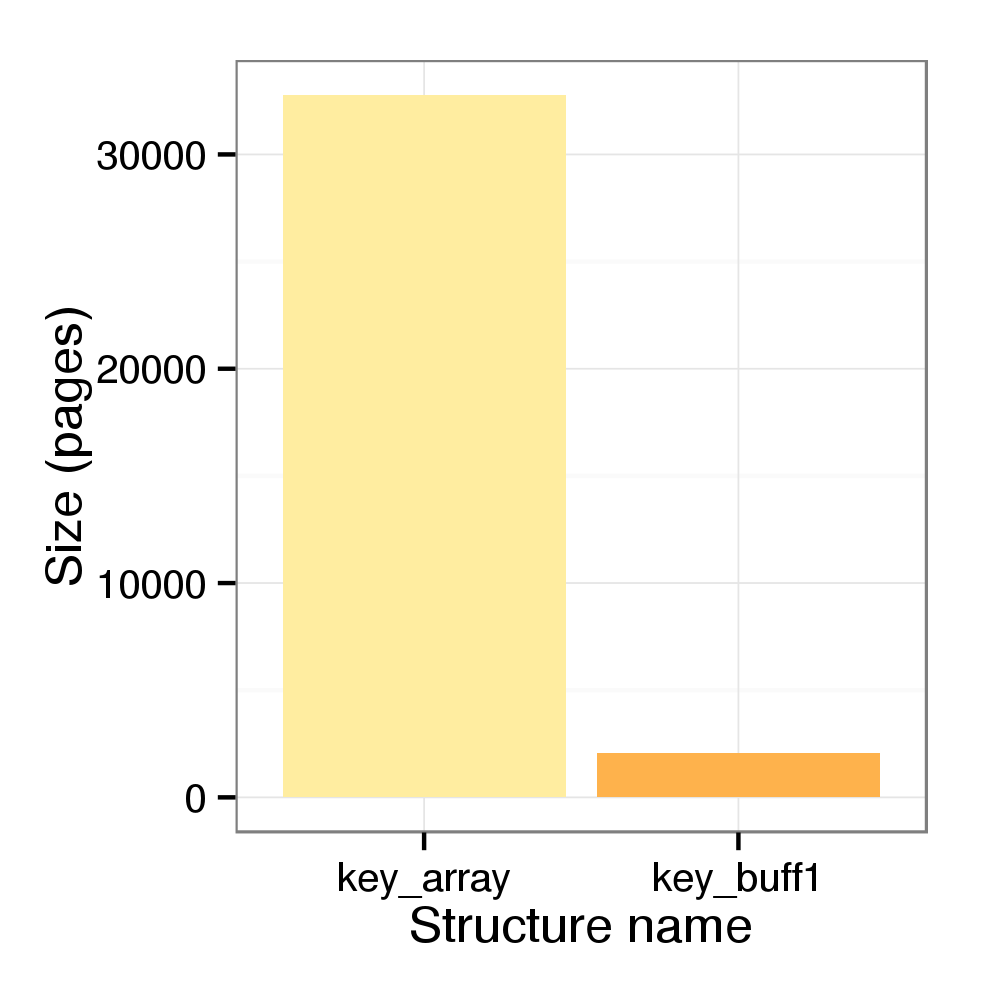
\includegraphics[width=\linewidth]{tabarnac/example_sz}
        \caption{Structures size.}
        \label{fig:example_sz}
    \end{subfigure}
    \begin{subfigure}{.49\linewidth}
        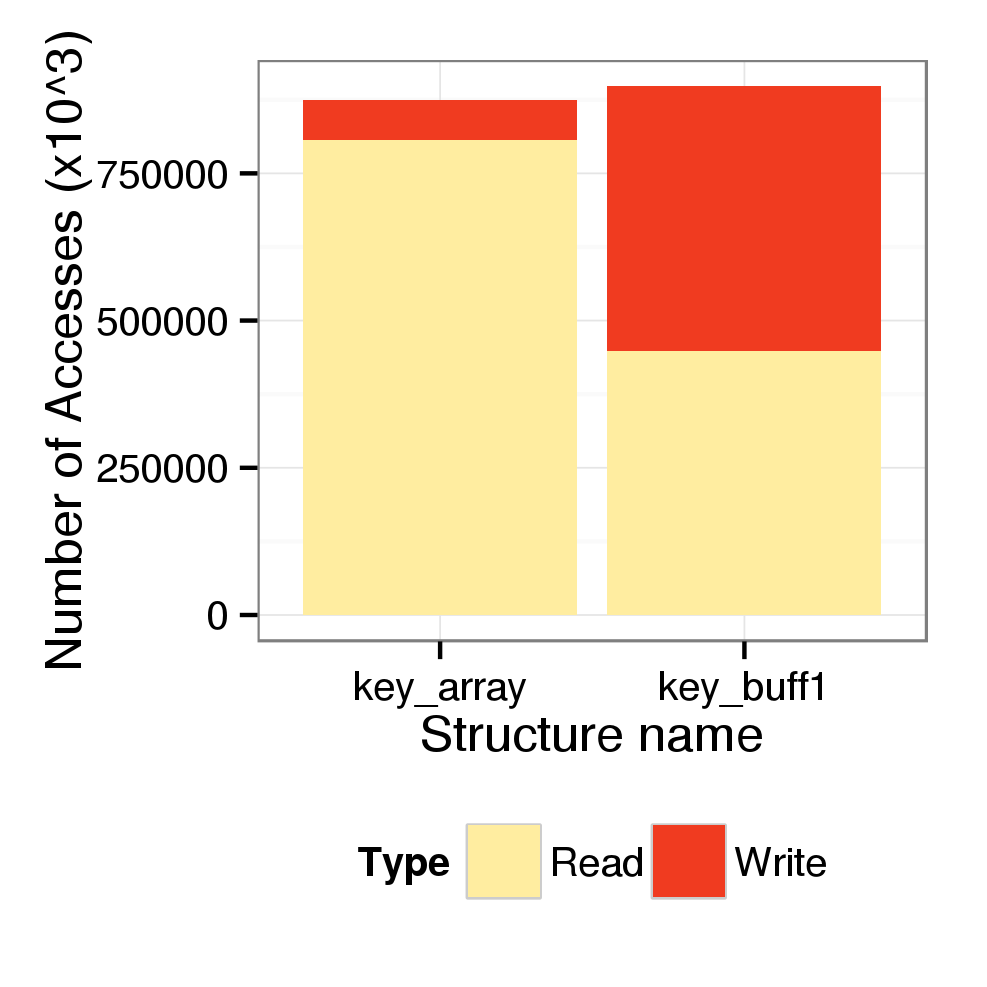
\includegraphics[width=\linewidth]{tabarnac/example_rw}
        \caption{Number of accesses per structures.}
        \label{fig:example_rw}
    \end{subfigure}
    \caption{Global views of the memory usage.}
    \label{fig:example_plot1}
\end{figure}

The first series of plots presents information about the relative importance of the data structures.
It consists of two plots, showing the size of each data structure, as in Figure~\ref{fig:example_sz}, and the number of reads and writes in each structure as in Figure~\ref{fig:example_rw}.
These plots give a general idea of the importance of the structures used by the parallel application.
Moreover, knowing the global read/write distribution is very useful as it determines the possible optimizations.
For instance, small data structures written only during initialization or very rarely can be relatively easily
duplicated, such that each \gls{NUMA} node works on a local copy.

\begin{figure}[htb]
    \centering
    \begin{subfigure}{.49\linewidth}
        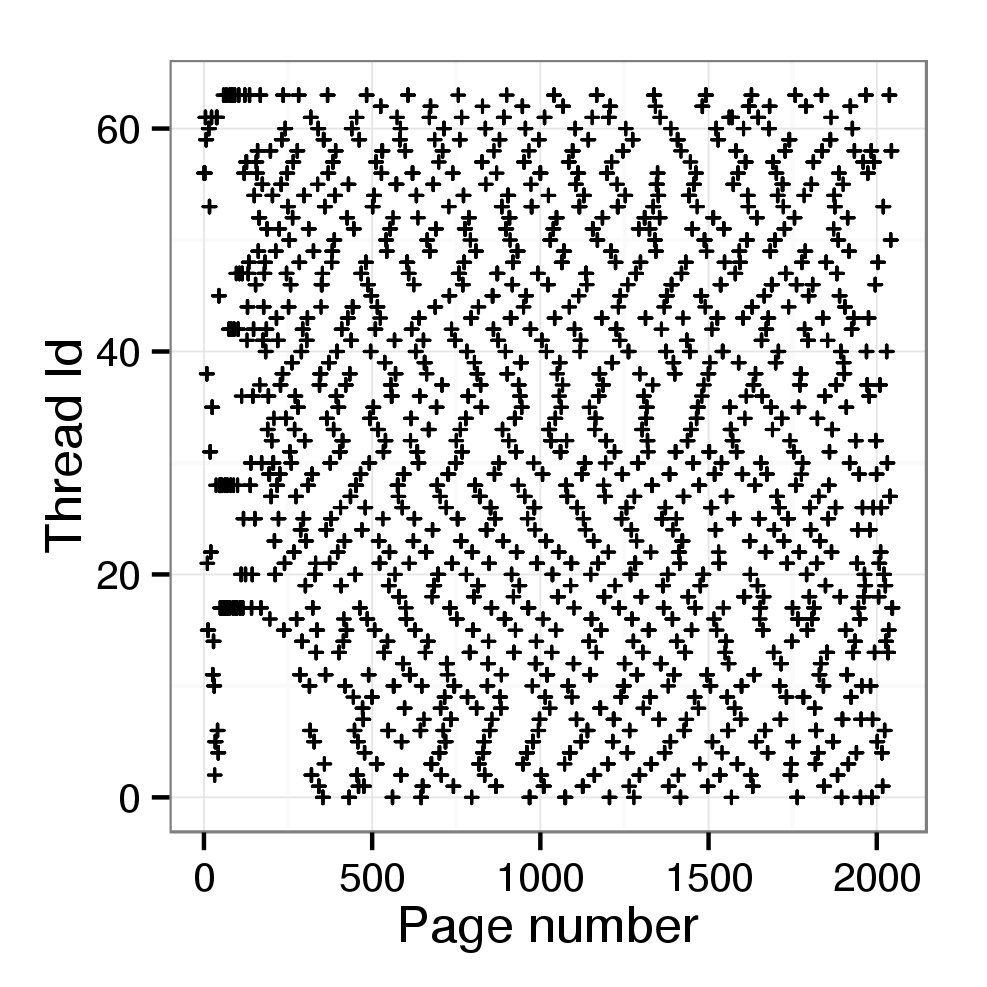
\includegraphics[width=\linewidth]{tabarnac/example_ft}
        \caption{First touch distribution.}
        \label{fig:example_ft}
    \end{subfigure}
    \begin{subfigure}{.49\linewidth}
        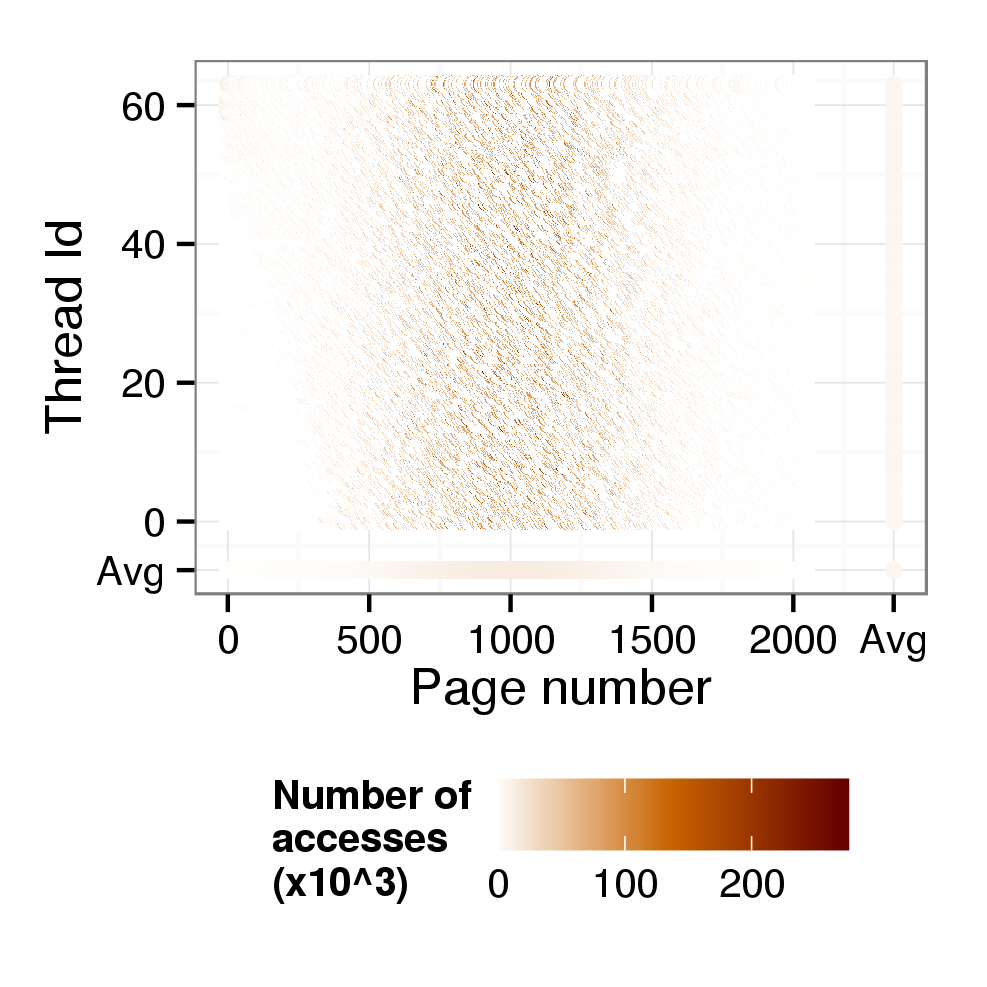
\includegraphics[width=\linewidth]{tabarnac/example_dist}
        \caption{Per thread access distribution.}
        \label{fig:example_dist}
    \end{subfigure}
    \caption{Per structure view of the memory usage.}
    \label{fig:example_by_structs}
\end{figure}

The second series of plots is the most important one.
It shows, for each page of each structure, which thread is responsible for the first touch (Figure~\ref{fig:example_ft}).
This information is important as the default policy for \gls{Linux} and most other operating systems is to map a page as close as possible to the first thread accessing it.
If the first touch distribution does not fit the overall access distribution, the default mapping performed by \gls{Linux} might not be efficient.
To address this issue, the developer can either correct the first touch or do some manual data mapping to ensure better memory access locality and balance during the execution.

This second series also shows the density of accesses performed by each thread and their global distribution.
In the example shown in \fig{example_dist}, each horizontal line represents the number of accesses performed by each thread to the memory space.
There is also one line for the average number of accesses.
Additionally, for each thread the average number of accesses to the structure is indicated by its tone.
Darker points indicate more memory accesses to the page. This visualization gives an easy way to understand the data sharing between threads, as well as the balance between pages and
threads.
These plots can be used to identify inefficient memory sharing and to determine the best \gls{NUMA} mapping policy.
For instance in \fig{example_dist}, we can see that the addresses in the middle of the data structure (from 500 to 1500) are accessed by each threads and significantly more than the other pages.
The consequences on the performances of this pattern and how we can improve it are discussed in \sect{tab-is}.

\section{Experimental validation}
\label{sec:tab-expe}

To evaluate \gls{Tabarnac}, we present two examples of benchmark optimization achieved with the help of \gls{Tabarnac}.
For each benchmark, we compare the speedup obtained with the modifications done using the knowledge provided by \gls{Tabarnac} to the one obtained by using several classic \gls{NUMA} mapping tools and policies.
We also evaluate the overhead of \gls{Tabarnac} on each of the \gls{NPB}.

\subsection{Methodology}

%This section briefly discusses our experimental setup for the evaluation of \gls{Tabarnac}.
% and presents relevant information on the experimental environment.
%presents the hardware architecture, the mapping policies to which we compare
%pour propositions, and the other relevant environment informations.

\begin{table}[htb]
    \centering
    \begin{tabular}{lccccc}
        \toprule
        & \multicolumn{5}{c}{\textbf{Hardware totals}}\\
        \cmidrule(lr){2-6}
        & Nodes & Threads & Vendor & Model & Memory \\
        \cmidrule(lr){2-6}
        \texttt{Turing}   & $4$ & $64$ & Intel & Xeon X7550   & \SI{128}{Gib} \\
        \texttt{Idfreeze} & $8$ & $48$ & AMD   & Opteron 6174 & \SI{256}{Gib}\\
        \midrule
        & \multicolumn{5}{c}{\textbf{Hardware per node}}\\
        \cmidrule(lr){2-6}
        & Cores & Threads & Frequency & L3 Cache & Memory \\
        \cmidrule(lr){2-6}
        \texttt{Turing}   & $8$ & $16$ & \SI{2.00}{Ghz}& \SI{18}{Mib} & \SI{32}{Gib} \\
        \texttt{Idfreeze} & $6$ & $6$  & \SI{2.20}{Ghz}& \SI{12}{Mib} & \SI{32}{Gib}\\
        \midrule
        & \multicolumn{5}{c}{\textbf{Software}}\\
        \cmidrule(lr){2-6}
        & Kernel & \multicolumn{2}{c}{Distribution} &
            \multicolumn{2}{c}{Bios configurations} \\
        \cmidrule(lr){2-6}
        \texttt{Turing}   & Linux 3.13 & \multicolumn{2}{c}{Ubuntu 12.04} &
            \multicolumn{2}{c}{Hyper threading} \\
        \texttt{Idfreeze} & Linux 3.2 & \multicolumn{2}{c}{Debian Jessie} &
            \multicolumn{2}{c}{No hyper threading}\\
        \bottomrule
    \end{tabular}
    \caption{Hardware and software configuration of the evaluation systems for Tabarnac.}
    \label{tab:turing-hw}
\end{table}

We used two NUMA machines for our experiments, \texttt{Turing} and \texttt{Idfreeze}.
The second machine has only been used to compare the instrumentation overhead between Intel and AMD machines.
All the other experiments ran on \texttt{Turing}.
The hardware and software configurations are summarized in \tbl{turing-hw}.

We evaluated the overhead of \gls{Tabarnac} over all the~\cite{Jin99NPBOpenMP}.
Moreover we present the performance optimization of the following applications with \gls{Tabarnac}: the \IS benchmark from the \gls{NPB} and \Ondes.
They were chosen to demonstrate different memory access behaviors with different strategies to improve them.

All applications use OpenMP for parallelization, they were compiled with \texttt{gcc}, version 4.6.3, with the \texttt{-O2} optimization flag.
Both analysis and performance evaluation are performed with the maximum number of threads that the machine can manage with its hardware, which means $64$ threads for \texttt{Turing} and $48$ for \texttt{Idfreeze}.

For the application we modified thanks to the knowledge obtained with \gls{Tabarnac}, we also compare the performances obtained with following two traditional mapping policies.
The \emph{interleave} policy is performed with the help of the \texttt{numactl} tool~\cite{Kleen05NUMA}.
The recently introduced \emph{NUMA Balancing} technique~\cite{Corbet12Toward}, which is executed with its default configuration.
Our baseline for the experiment is an unmodified Linux kernel, version $3.13$, with the first-touch policy.
The NUMA Balancing mechanism is disabled in this baseline.
To lessen the overhead of \gls{Tabarnac}, we analyzed the applications with smaller input than the one used for their performance analysis.

For the plots presenting speedups, each configuration was executed at least $10$ times.
Each point shows the arithmetic mean of all runs.
The error bars in those plots represent the standard error.

All the files required to reproduce the experiments  or the analysis described here online: \url{https://github.com/dbeniamine/tabarnac\_expe}.

\subsection{Ondes3D}
\label{sec:tab-ondes3d}

\Ondes is the main numerical kernel of the Ondes3D application~\cite{Dupros08Exploiting}.
It simulates the propagation of seismic waves using a finite differences numerical method.
We analyzed \Ondes with \gls{Tabarnac} on a small input resulting in \SI{0.7}{Gib} of memory usage.
For the performance analysis, we increased the size of the input reaching \SI{11.3}{Gib} of memory used.

\begin{figure}[htb]
    \centering
    \begin{subfigure}{.49\linewidth}
        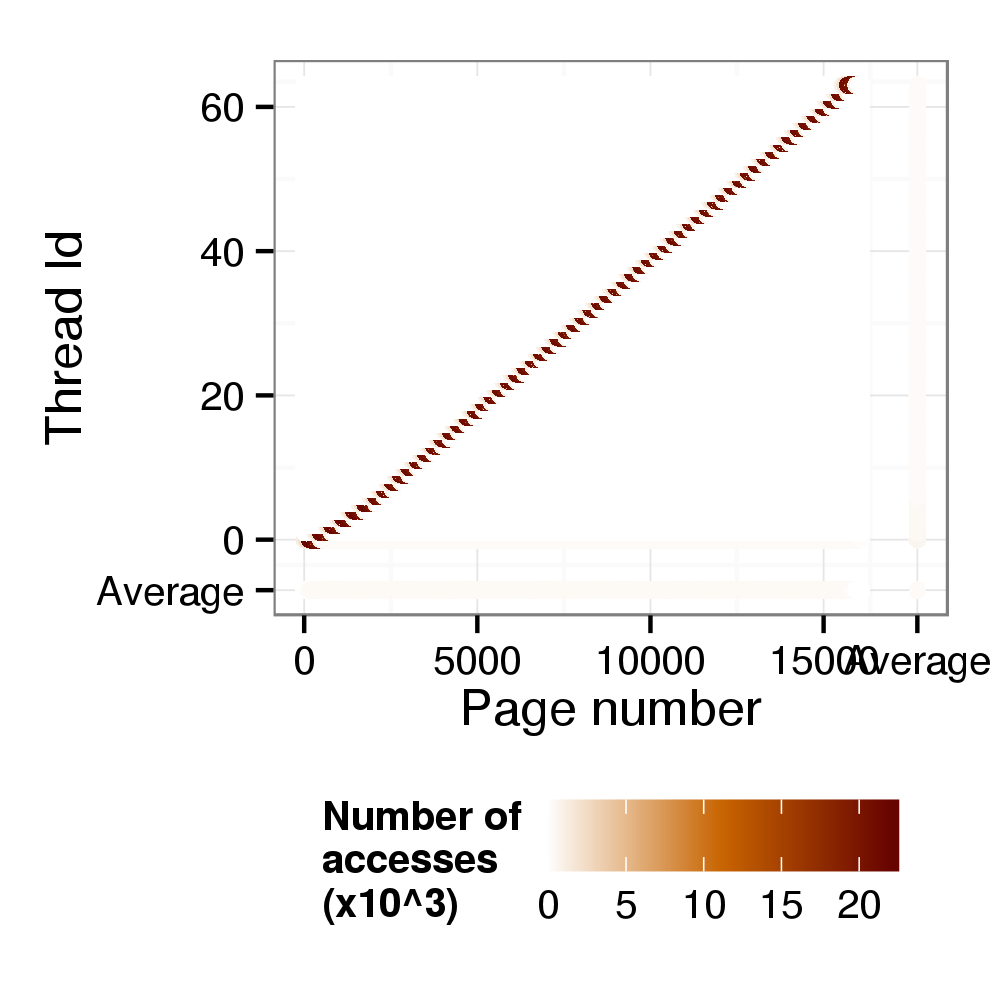
\includegraphics[width=\linewidth] {tabarnac/ondes3d_vz0_dist_orig}
        \caption{Access distribution}
        \label{fig:ondes3d-behaviour-vz0-orig}
    \end{subfigure}
    \newline
    \begin{subfigure}{.49\linewidth}
        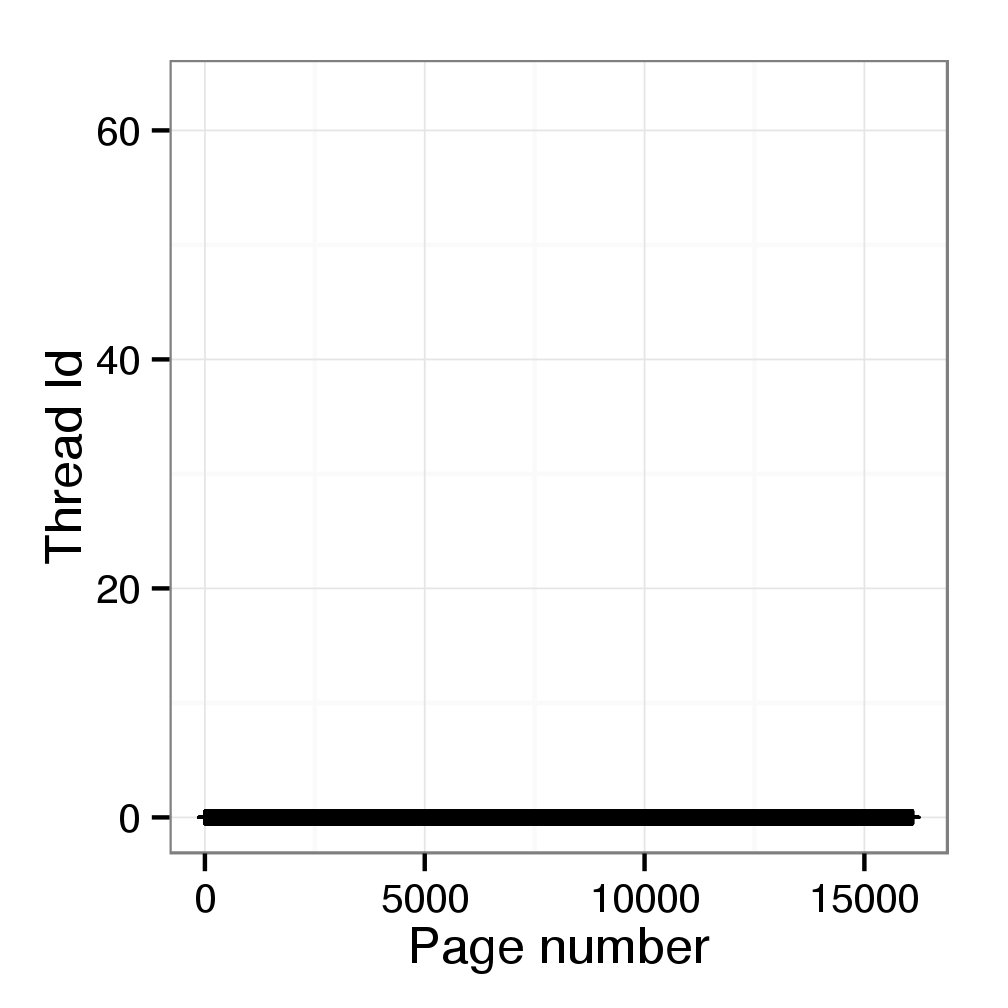
\includegraphics[width=\linewidth] {tabarnac/ondes3d_vz0_ft_orig}
        \caption{Original first-touch.}
        \label{fig:ondes3d-ft-vz0-orig}
    \end{subfigure}
    \begin{subfigure}{.49\linewidth}
        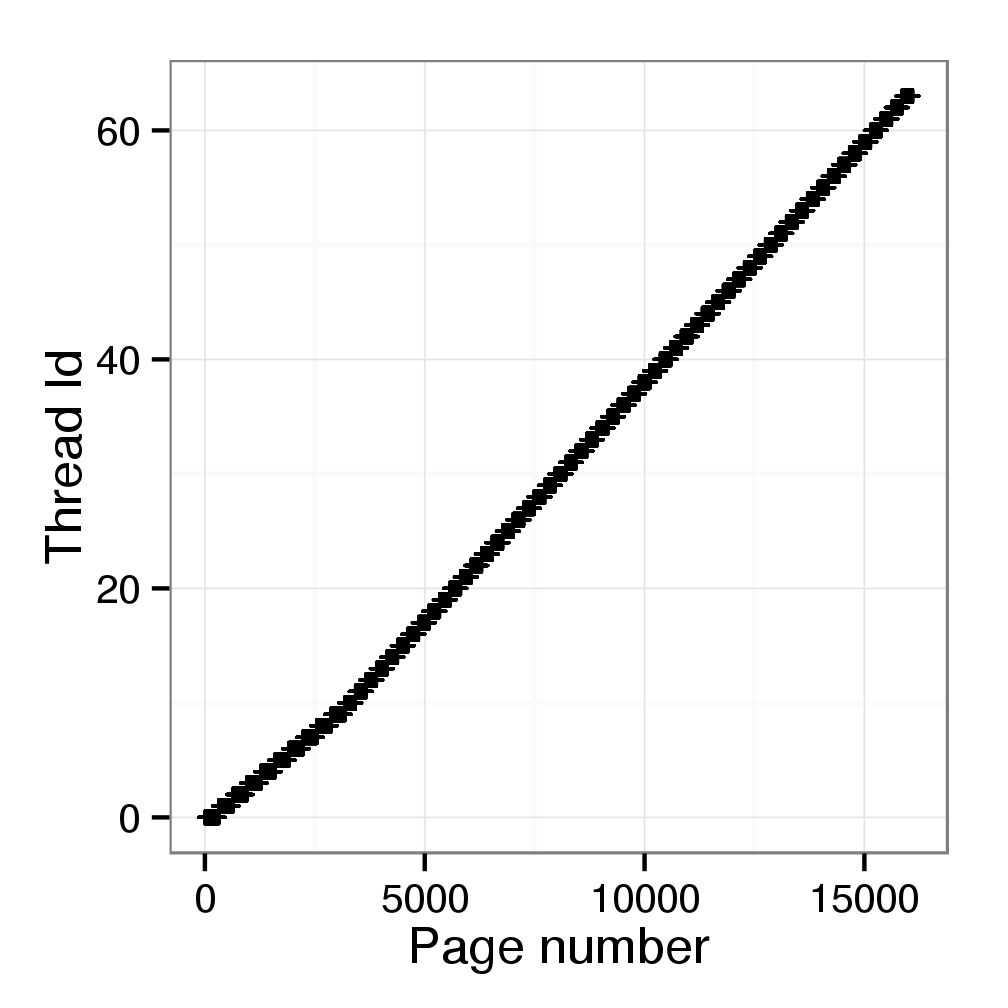
\includegraphics[width=\linewidth] {tabarnac/ondes3d_vz0_ft_modif}
        \caption{Improved first-touch.}
        \label{fig:ondes3d-ft-vz0-modif}
    \end{subfigure}
    \caption{Access distribution and first-touch for structure
        \texttt{vz0} from \Ondes.} %Original version on the left,
    %modified on the right.}
    \label{fig:ondes3d}
\end{figure}

The analysis of the accesses distribution in \Ondes shows that each structure seems to be well distributed between the threads, as we can see for structure \texttt{vz0} in \fig{ondes3d-behaviour-vz0-orig}.
However, for all structures, thread~$0$ is responsible for all first accesses, as we can see in \fig{ondes3d-ft-vz0-orig}.
Due to this pattern, if we run \Ondes without any improved mapping policy, every page will be mapped to the \gls{NUMA} node that executes the thread~$0$, resulting in remote
accesses for the other threads.
An easy fix is to perform the initialization in parallel and to pin each thread on a different core.
Such a modification results in the first touch distribution shown in \fig{ondes3d-ft-vz0-modif}, for which pages are distributed among all the threads.

\begin{figure}[htb]
    \centering
    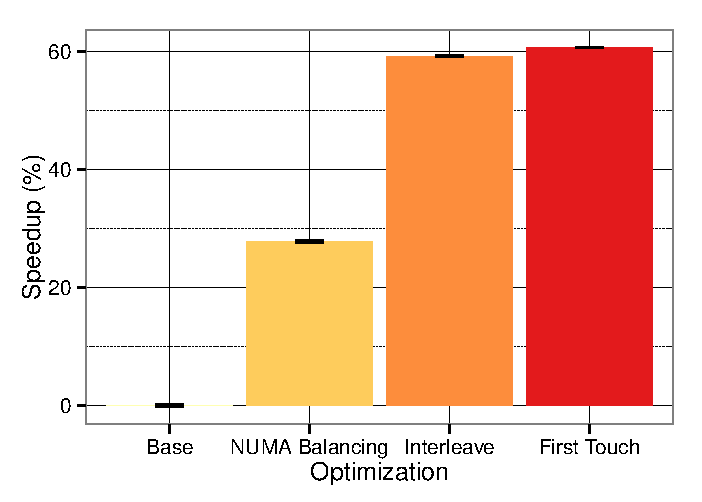
\includegraphics[width=.8\linewidth]{tabarnac/ondes3d_exectime}
    \caption[Speedup for \Ondes.]{Speedup for \Ondes compared to the baseline.}
    \label{fig:ondes-res}
\end{figure}

We compare the performance of our modified version called \emph{First Touch} to three variants:
\begin{itemize}
    \item The original (\emph{Base}) version running on the unmodified \gls{OS}.
    \item A version using \emph{NUMA Balancing} to move pages online.
    \item A version with \emph{Interleave} policy that aims at reducing the impact of remote accesses.
\end{itemize}
\fig{ondes-res} present the results of this evaluation.
We can see that all methods improve the execution time compared to the base.
Still, but \emph{NUMA Balancing} provides less than \SI{30}{\%} speedup, while the static mappings (Interleave and the modified code) increase performance by \SI{60}{\%}.
Indeed, with \emph{NUMA Balancing}, all pages are initially mapped by the \gls{OS} to the \gls{NUMA} node of thread~$0$, and are only moved later on, after several remote accesses have already occurred, losing some optimization opportunities.
This is a case where static mapping can be substantially better than automated tools.
The \emph{Interleave} policy provides a similar speedup as \emph{First Touch} since it distributes the pages over the \gls{NUMA} nodes at the beginning of the execution.
In the end, for this example, using a classic static policy would have been enough to fix the performance issue, yet \gls{Tabarnac} helped understanding and fixing it in a definitive way.

\subsection{The \IS benchmark}
\label{sec:tab-is}

According to the \gls{NPB} website\footnote{\url{http://www.nas.nasa.gov/publications/npb.html}}, \IS has a random memory access pattern, although we observed a very specific pattern.
In this section we explain this pattern and how we used the knowledge about this pattern to improve the performance of \IS.

\IS was executed with input class \emph{D} for the performance evaluation, resulting in a memory usage of \SI{33.5}{Gib}, and class \emph{B} for the analysis, with a memory usage of \SI{0.25}{Gib}.

\begin{figure}[htb]
    \centering
    \begin{subfigure}{.4\linewidth}
        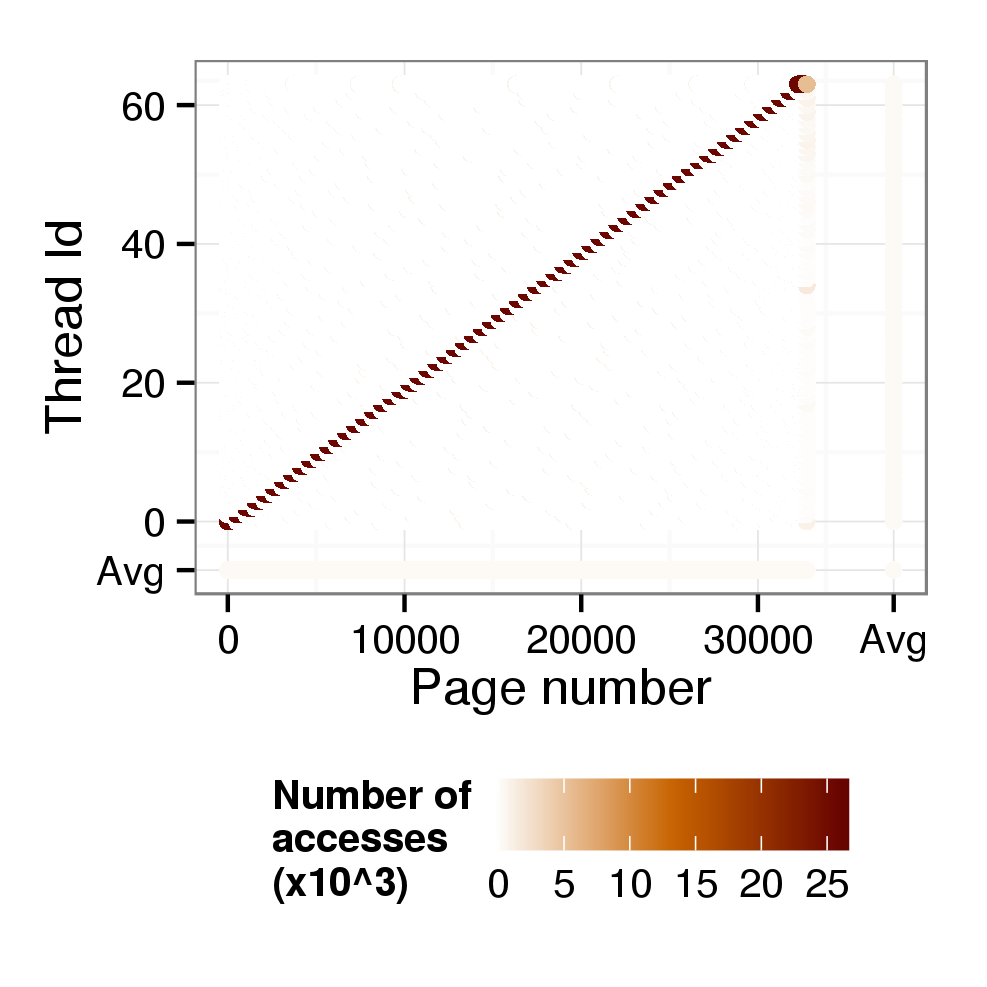
\includegraphics[width=\linewidth]  {tabarnac/is_b_kba_orig}
        \caption{\texttt{key\_array}.}
        \label{fig:is-behaviour-orig-kba}
    \end{subfigure}
    ~
    \begin{subfigure}{.4\linewidth}
        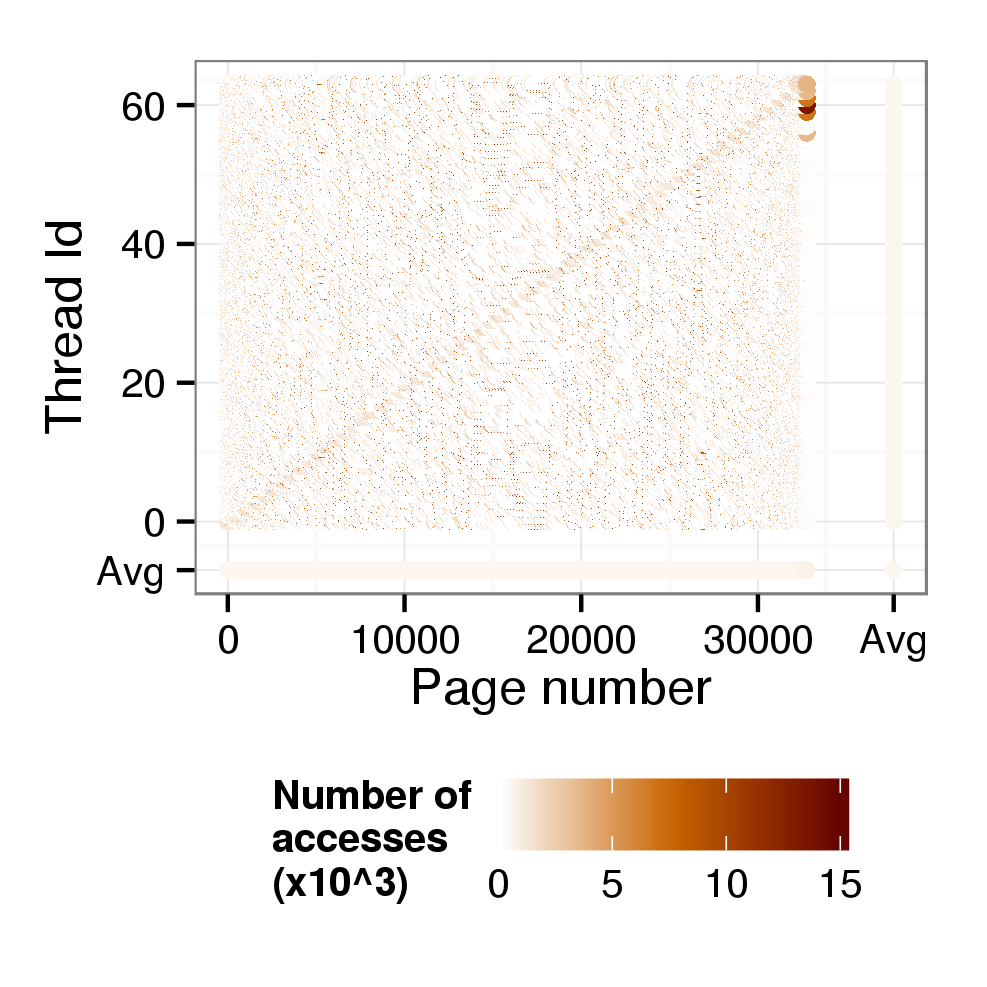
\includegraphics[width=\linewidth]  {tabarnac/is_b_kb2_orig}
        \caption{\texttt{key\_buff2}.}
        \label{fig:is-behaviour-orig-kb2}
    \end{subfigure}
    \begin{subfigure}{.4\linewidth}
        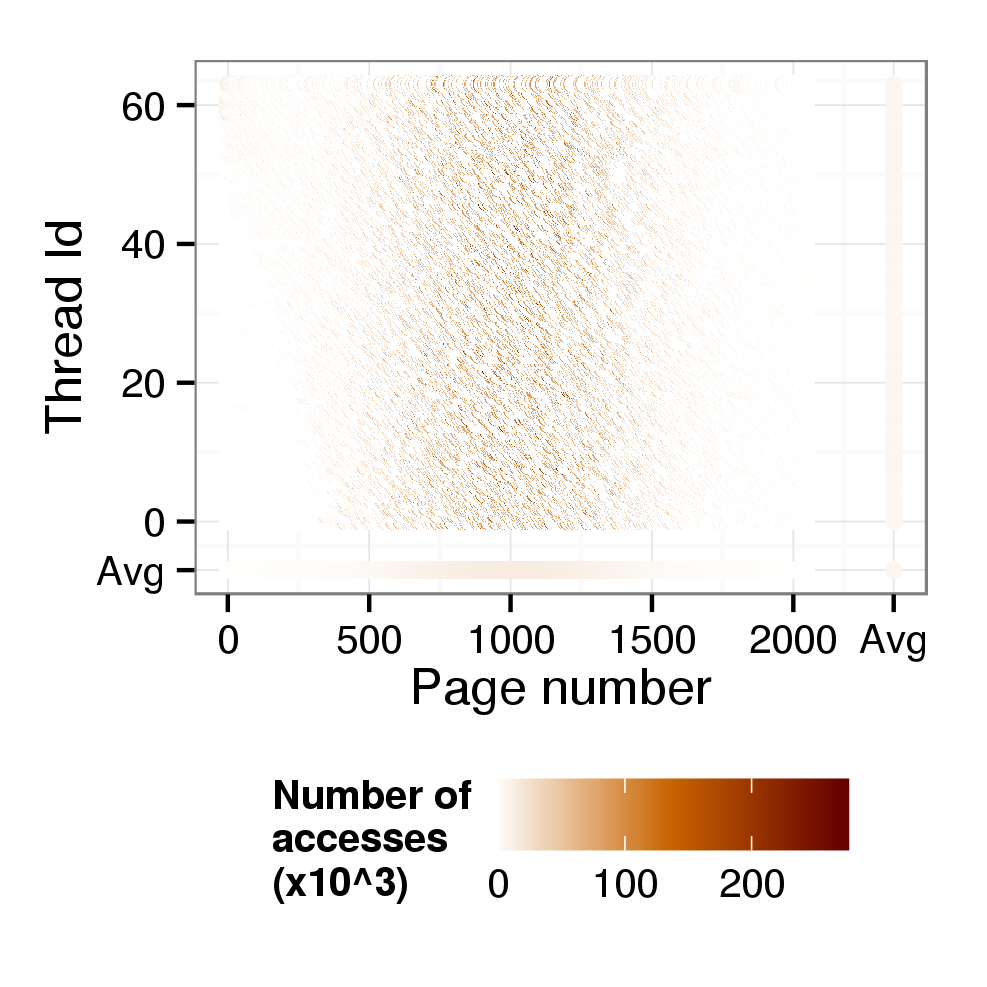
\includegraphics[width=\linewidth]  {tabarnac/is_b_kb1_orig}
        \caption{\texttt{key\_buff1}.}
        \label{fig:is-behaviour-orig-kb1}
    \end{subfigure}
    \caption[Original memory access distribution for \IS.]{Original memory access distribution for the main structures of \IS.}
    \label{fig:is-behaviour-orig}
\end{figure}

\fig{is-behaviour-orig} shows the original access distributions for the three main structures of \IS.
We can see that each structure has a different access pattern: for \texttt{key\_array} (\fig{is-behaviour-orig-kba}) each thread works on a different part of the structure, which let automated tools perform an efficient data/thread mapping on it.
On the other hand, \texttt{key\_buff2} (\fig{is-behaviour-orig-kb2}) is completely shared by all threads, we can barely see a diagonal pattern, indicating a small affinity between some threads and some pages.
\texttt{key\_buff1}'s access distribution (\fig{is-behaviour-orig-kb1}) is the most interesting one.
We can see that almost all accesses occur in pages in the middle of the structure (from page $500$ to $1500$), and those pages are shared by all threads.
This means that the number of access per page  for each thread follows a Gaussian distribution centered in the middle of the structure.

\lstinputlisting[caption={[Original IS code.]\IS code responsible for the distribution of memory accesses.}, label=lst:is, float=htb]{code/is.c}

We can identify the source of this pattern in the \IS source code.
Indeed, all the accesses to \texttt{key\_buff1} are linear, except the ones shown in \lstr{is}, Line~\ref{lst:is-gaus-end}, which depend on the values of \texttt{key\_buff2}\footnote{
    The code has been slightly modified to make it more readable.
    In the original version, the arrays generic pointers.
    Furthermore we removed several lines of code inside the loop that are not required to understand the memory pattern.
    }.
Those accesses happens in an \gls{OpenMP} parallel loop that has the particularity to be scheduled dynamically.
The comments on the \IS code explains that the values of \texttt{key\_buff2} follows a Gaussian distribution, therefore using a dynamic scheduling provides a good load balancing between the threads, while a cyclic distribution would results in some threads generating significantly more memory accesses than the others.
Still it is possible to use a cyclic scheduling instead of the default one (dynamic) by defining a variable at the compilation time.

\begin{figure}[htb]
    \centering
    \pgfmathdeclarefunction{gauss}{1}{%
    \pgfmathparse{1/(1.4*sqrt(2*pi))*exp(-((#1-4)^2)/(2*1.4^2))}%
}

%Palette 4-class paired
\definecolor{Col0}{HTML}{A6CEE3}
\definecolor{Col1}{HTML}{1F78B4}
\definecolor{Col2}{HTML}{B2DF8A}
\definecolor{Col3}{HTML}{33A02C}

\begin{tikzpicture}
\begin{axis}[
        axis x line=bottom,
        axis y line=left,
        xtick=\empty,
        ytick=\empty,
        ylabel={Intensity of accesses},
        xlabel={Page number},
        ymin=-.01,
        xmin=-.1,
        xmax=8.1,
        legend style={at={(1.1,1)}, anchor= north east}
     ]
    \addplot[name path=f,domain={0:8},forget plot] {gauss(x)};
    \addplot[name path=x,domain={0:8},forget plot] {0};
    \pgfplotsinvokeforeach{0,...,3}{
        \addplot[dashed,forget plot] coordinates {(#1+4,0) (#1+4,{gauss(#1+4)})};
        \addplot[dashed,forget plot] coordinates {(#1,0) (#1,{gauss(#1)})};

        \addplot[color= Col#1,forget plot] fill between[of=f and x,
            soft clip={(#1,0) rectangle (#1+1,1) },];
            \addplot[color= Col#1] fill between[of=f and x,
            soft clip={(#1+4,0) rectangle (#1+5,1)},];
        \addlegendentry{Thread #1}
    }

    \addplot[solid,very thick,white] coordinates {(4,0) (4,{gauss(4)})};
\end{axis}
\end{tikzpicture}

    \caption{Fair distribution of the pages of \texttt{key\_buff2} among the threads.}
    \label{fig:is-fair}
\end{figure}

\begin{lstlisting}[caption={Modified IS code.}, label=lst:is-modif,float=htb]
#pragma omp for schedule(static,NUM_BUCKETS/
    (2*omp_get_num_threads()))
\end{lstlisting}

As simple cyclic distribution of the loop would result in unbalanced work, we can design a slightly more complex distribution that provides a fair load balancing while enforcing locality of data.
To do so, we split the loop into two equal parts and distribute each part among the threads in a cyclic way  as shown in \fig{is-fair} where each color represent a thread.
This can be done by modifying the \gls{OpenMP} pragma (Line~\ref{lst:is-sched} in the original code), as shown in \lstr{is-modif}.
Obviously this distribution does not provide an optimal load balancing, but only a relatively fair one.

\begin{figure}[htb]
    \centering
    \begin{subfigure}{.4\linewidth}
        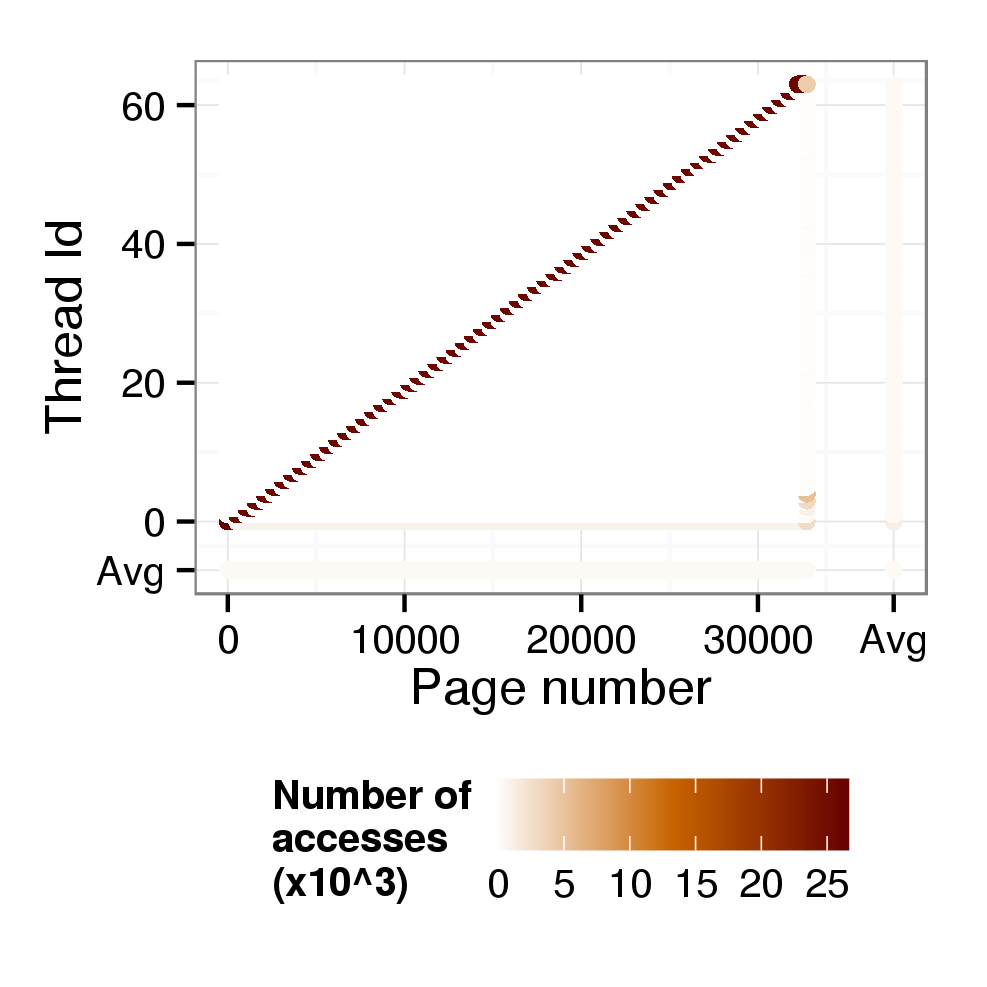
\includegraphics[width=\linewidth] {tabarnac/is_b_kba_modif}
        \caption{\texttt{key\_array}.}
        \label{fig:is-behaviour-modif-kba}
    \end{subfigure}
    ~
    \begin{subfigure}{.4\linewidth}
        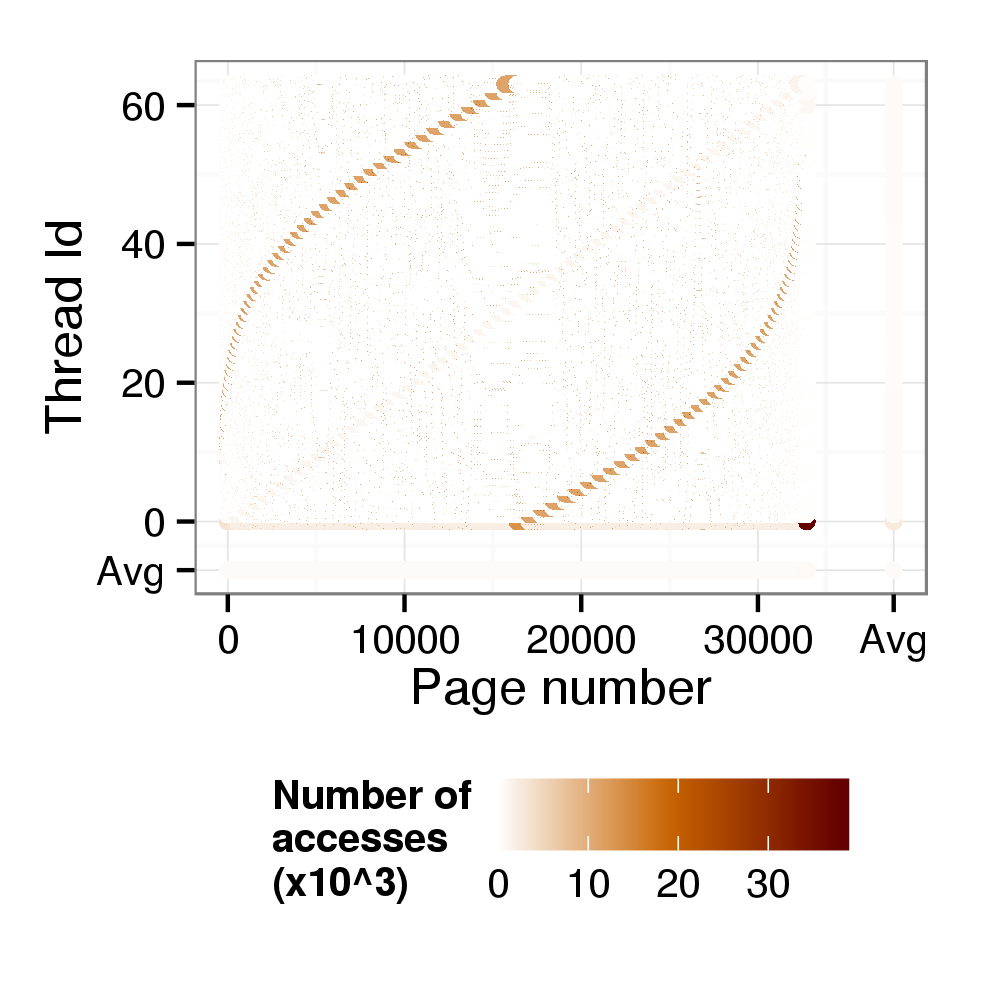
\includegraphics[width=\linewidth] {tabarnac/is_b_kb2_modif}
        \caption{\texttt{key\_buff2}.}
        \label{fig:is-behaviour-modif-kb2}
    \end{subfigure}
    \begin{subfigure}{.4\linewidth}
        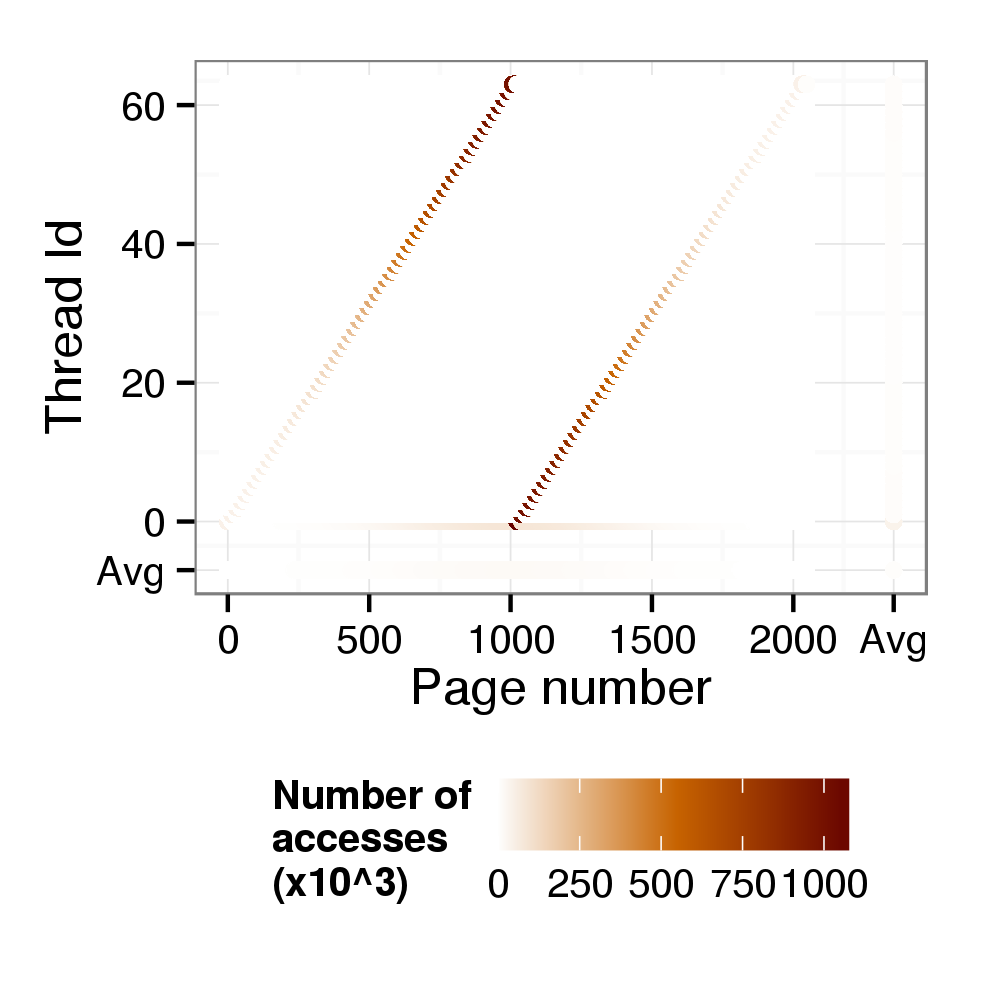
\includegraphics[width=\linewidth] {tabarnac/is_b_kb1_modif}
        \caption{\texttt{key\_buff1}.}
        \label{fig:is-behaviour-modif-kb1}
    \end{subfigure}
    \caption[Modified memory access distribution for \IS.]{Modified memory access distribution for the main structures of \IS.}
    \label{fig:is-behaviour-modif}

\end{figure}

\fig{is-behaviour-modif} show the accesses distribution obtained with this code modification.
We can see that now each thread accesses a different part of \texttt{key\_buff1}.
Furthermore, if most of the accesses still occur in the middle of the structure, the average number of accesses across the whole structure is the comparable same for all threads, which means that our distribution preserves the good load balancing.
Our modification has also changed \texttt{key\_buff2}'s accesses distribution.
Indeed, we can now clearly see a sharing pattern very similar to the one obtained for \texttt{key\_buff1}.

The main point of our code modification is to improve the affinity between thread and memory, therefore we need to pin each thread on a core to keep them close to the data they access.
To perform the thread mapping, we use the \texttt{GOMP\_CPU\_AFFINITY} environment variable.
\gls{Tabarnac} also showed us that the first touch is always done by the thread actually using the data for IS, therefore we do not need to explicitly map the data to the \gls{NUMA} nodes.

We compare the execution time of \IS (class \emph{D}) for the three scheduling methods, \emph{Dynamic}, \emph{Cyclic} and our custom \emph{Fair} distribution.
We evaluated each scheduling method in each of the following setup: with our \emph{Base} unmodified \gls{OS}, with the \emph{Interleave} policy and with \emph{Numa Balancing} activated.
As our modification rely on the firs-touch it does not make sense with Interleave and \gls{NUMA} Balancing, therefore these policies are not evaluated for our \emph{Fair} distribution.

\begin{figure}[htb]
    \centering
    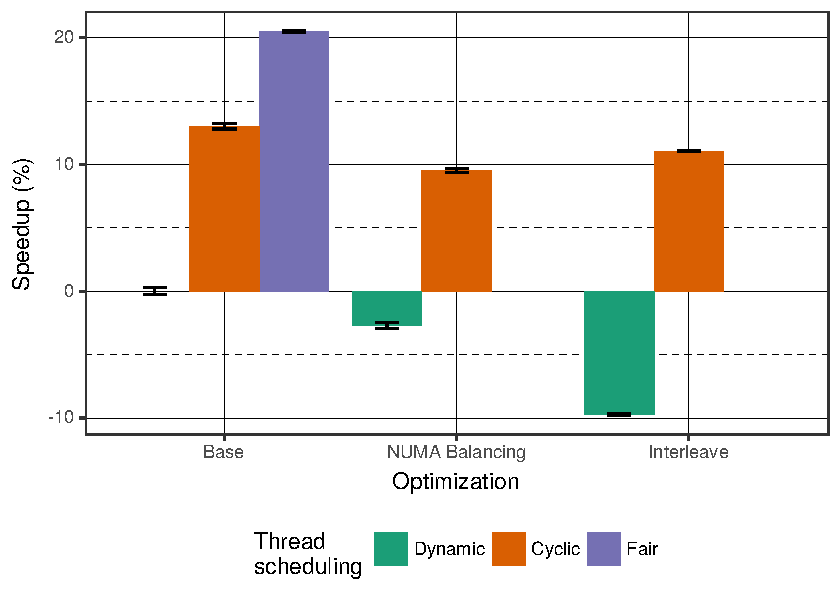
\includegraphics[width=\linewidth]{tabarnac/is_exectime}
    \caption[Speedup for \IS.]{Speedup for \IS (class D) compared to the baseline.}
\label{fig:is-res}
\end{figure}

\fig{is-res} shows the speedup of \IS compared to the default version (\emph{Dynamic}) for each scheduling method and for each mapping policy.
The first thing to notice is that with the default \emph{Dynamic} scheduling, both Interleave and \gls{NUMA} Balancing slow the application down, by up to \SI{10}{\%}.
This slowdown is due to the fact that two mechanisms (the mapping policy and the \gls{OpenMP} runtime) or modifying the application behavior with conflicting interests and without communicating.
Then we can note that \emph{Cyclic} scheduling, proposed in the original code, already provides up to \SI{13}{\%} of speedup.
Yet, both interleave and \gls{NUMA} Balancing are still reducing the performance gains.
Finally, the \emph{Cyclic-Split} version provides more than \SI{20}{\%} of speedup with a very small code modification.
This example shows that while mapping policies (static or dynamic) can conflict with the parallel runtime and slow the execution time, analyzing an application's memory behavior can help fixing inefficient behavior resulting in significant performances gain.

\subsection{Tracing overhead}

Finally,  we evaluate the instrumentation cost of \gls{Tabarnac}.
To do so, we executed all of the \gls{NPB} in class \emph{B}\footnote{
    \DC was run in class \emph{A} as it was too slow in class \emph{B} to run the full experiment.
} with $64$ threads on both evaluation systems and compared the original execution time to the execution time with instrumentation enabled.

\begin{figure}[htb]
    \centering
    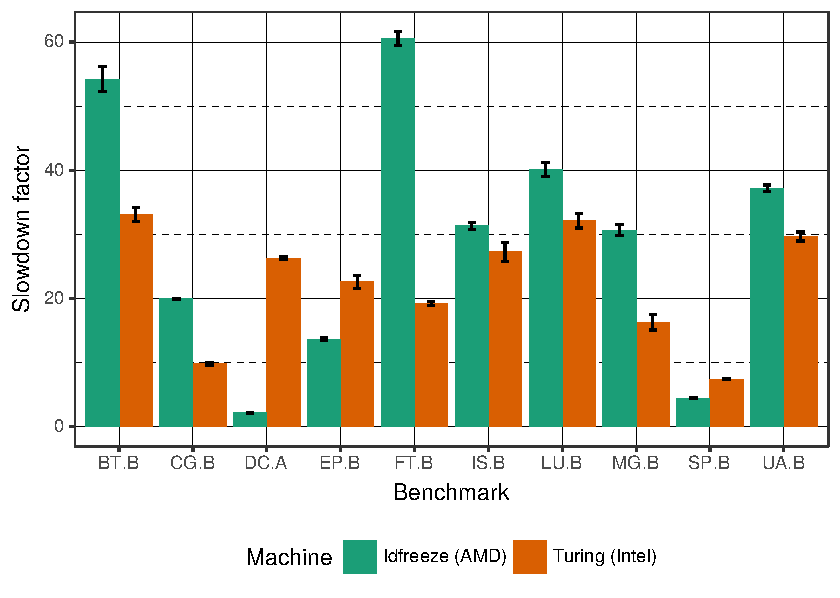
\includegraphics[width=\linewidth]{tabarnac/tool-ovh.pdf}
    \caption{Tabarnac's instrumentation overhead.}
    \label{fig:ovh-tabarnac}
\end{figure}

As we can see in \fig{ovh-tabarnac}, on the Intel machine, the instrumentation slows the execution down by a factor ranging from $10$ to $30$.
Nevertheless, on the \gls{AMD} machine, the instrumentation is $10$ to \SI{50}{\%} slower for most benchmarks, and two to three times slower than on the \gls{Intel} machine for pathological cases.
This behavior was expected as \gls{Pin} is an instrumentation library developed by \gls{Intel}.
Although this overhead is not negligible, we have to consider the fact that often we can instrument smaller versions of the applications, as we focus on the general behavior.
Moreover, our method is more precise than sampling and thus one run is often enough.
Finally, as our analysis is designed to be used during the development phase and not at runtime in an automated tool, we consider that this overhead is acceptable.


\section{Results and discussion}
\label{sec:tab-cncl}

Our experiments have highlighted the fact that using blindly static mapping policies such as Interleave or dynamic tools such as \gls{NUMA} Balancing can result in significant performance loss.
Furthermore in the experiments where both dynamic and static policies increased the performances, the difference between the gain provided by the two policies was significant.
The only way to predict which tool is the most suited to an application is to understand the sharing patterns of the memory of this application by the threads.

\gls{Tabarnac} enables developers and users to achieve performance improvements in two ways.
First, by providing a deep understanding of the memory sharing pattern, it enables the user to find the best existing mapping policy.
Second, this knowledge can be used to identify and fix inefficient memory behavior, for instance by designing a specific thread scheduling taking the sharing patterns into account.
Our experiments showed that both situations result in significant performance gains.

While \gls{Tabarnac} helps the developper identify and fix some inefficient sharing patterns, it only provides a global overview of the memory usage.
Indeed it does not collect any temporal information.
Therefore, it does not enable identification of the distribution of inefficient memory access patterns over the time, such as the ones depicted in \sect{archi} with the naïve matrix multiplication.

% vim: et si sta lbr  sw=4 ts=4 spelllang=en_us
